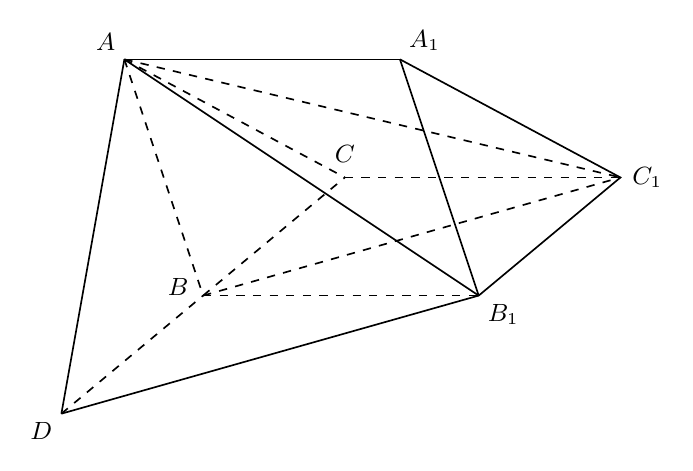
\begin{tikzpicture}[scale=1,line width=.6pt]
\tikzset{lbl/.style={font=\small,inner sep=1pt}}
\coordinate (A) at (0,4);
\coordinate (A1) at (3.5,4);
\coordinate (B) at (1,1);
\coordinate (B1) at (4.5000000000,1.0000000000);
\coordinate (C) at (2.8,2.5);
\coordinate (C1) at (6.3000000000,2.5000000000);
\coordinate (D) at (-0.8000000000,-0.5000000000);
% solid visible
\draw (A)--(A1);
\draw (A1)--(B1);
\draw (A)--(D);
\draw (D)--(B1);
\draw (A)--(B1);
\draw (A1)--(C1)--(B1);
% dashed hidden
\draw[dashed] (A)--(B);
\draw[dashed] (B)--(C);
\draw[dashed] (A)--(C);
\draw[dashed] (A)--(C1);
\draw[dashed] (B)--(B1);
\draw[dashed] (C)--(C1);
\draw[dashed] (B)--(C1);
\draw[dashed] (D)--(B);
\node[lbl,above left=2pt] at (A) {$A$};
\node[lbl,above right=2pt] at (A1) {$A_{1}$};
\node[lbl,left=3pt,xshift=-1pt,yshift=3pt] at (B) {$B$};
\node[lbl,below right=2pt] at (B1) {$B_{1}$};
\node[lbl,above=4pt] at (C) {$C$};
\node[lbl,right=3pt] at (C1) {$C_{1}$};
\node[lbl,below left=2pt] at (D) {$D$};
\end{tikzpicture}